\documentclass[aspectratio=169,10pt]{beamer}

\usetheme{default}
\usecolortheme{default}
\setbeamertemplate{navigation symbols}{}
\setbeamertemplate{footline}[frame number]
\setbeamertemplate{itemize items}[circle]
\setbeamercolor{alerted text}{fg=blue!55!black}
\setbeamerfont{frametitle}{size=\large,series=\bfseries}

\usepackage{amsmath,amssymb,mathtools}
\usepackage{booktabs,array}
\usepackage{graphicx}
\usepackage{tabularx}
\usepackage{microtype}

\graphicspath{{assets/}}
\newcommand{\takeaway}[1]{\vfill{\footnotesize\textbf{Takeaway.} #1}}
\newcommand{\notfound}[1]{\textbf{[NUMBER NOT FOUND: #1]}}

\title{[PLACEHOLDER: Title TBD]}
\author{Tommaso De Santo}
\date{Draft for author assessment\\July 7, 2026}

\begin{document}

% 1
\begin{frame}{[PLACEHOLDER: the title claim is still to be written]}
  \titlepage
\end{frame}

% 2
\begin{frame}{The motivation pitch will connect housing access to fertility}
  \alert{[PLACEHOLDER: pitch]}
  \begin{itemize}
    \item [PLACEHOLDER: motivation fact 1]
    \item [PLACEHOLDER: motivation fact 2]
    \item [PLACEHOLDER: motivation fact 3]
  \end{itemize}
\end{frame}

% 3
\begin{frame}{The paper contribution statement is still a placeholder}
  \alert{[PLACEHOLDER: this paper]}
  \begin{itemize}
    \item [PLACEHOLDER: theory contribution]
    \item [PLACEHOLDER: quantitative contribution]
    \item [PLACEHOLDER: policy contribution]
  \end{itemize}
\end{frame}

% 4
\begin{frame}{The literature positioning will be filled after author review}
  \begin{itemize}
    \item [PLACEHOLDER: Sommer--Sullivan--Verbrugge slot]
    \item [PLACEHOLDER: Doepke--Kindermann slot]
    \item [PLACEHOLDER: Greaney--Parkhomenko--Van Nieuwerburgh (DUE) slot]
    \item [PLACEHOLDER: Couillard slot; Hacamo slot]
  \end{itemize}
\end{frame}

% 5
\begin{frame}{A two-period OLG links young fertility choices to old incumbent retention}
  Potential young households enter with income and wealth:
  \[
  i=(y_i,a_i),
  \]
  so entry wealth directly shapes access to owner housing.
  \begin{itemize}
    \item Young households choose entry, tenure, occupied housing, fertility, and saving.
    \item Young owners become old incumbents; old renters enter old age without housing.
    \item Old incumbents choose consumption, retained housing, and estates.
  \end{itemize}
  The tax wedge from sale rather than death is summarized by:
  \[
  \bar\ell=\tau^g\,\frac{P\,\varpi}{1+\varpi}
  \]
  Selling triggers the capital-gains tax, while death forgives it through basis step-up.
\end{frame}

% 6
\begin{frame}{Rental and finance frictions collapse into one family-housing cap}
  The owner cap is the smaller of the owner size limit and down-payment capacity:
  \[
  h_i\le
  H_i^O(q,\tau^p)
  =
  \min\left\{
  \bar h^O,
  \frac{a_i\rho}{(1-\phi)q}
  \right\}.
  \]
  The renter analog is $H_i^R=\bar h^R$, so tenure maps different primitives into one cap object.

  The child-cost display makes the cap's fertility price exact:
  \[
  \underbrace{\frac{\vartheta\,(c_i^m-\chi n_i^m)}{n_i^m}}_{\text{willingness to pay for a marginal child}}
  =
  \underbrace{\chi+\kappa(q^m+\zeta_i^m)}_{\text{full price of a child}} .
  \]
  A binding access constraint acts like a tax of $\kappa\zeta_i^m$ per child.
\end{frame}

% 7
\begin{frame}{The access gap is the goods value of relaxing constrained family space}
  For renters, the bundle reveals the cap bite:
  \[
  \frac{u^Y_{h,i}}{u^Y_{c,i}}
  =
  \frac{\alpha\,(c_i^R-\chi n_i^R)}{h_i^R-\kappa n_i^R}
  =
  q+\zeta_i^R.
  \]
  A renter at the size cap values another unit above market rent.

  For owners, the access gap separates finance from the owner size limit:
  \[
  \zeta_i^O
  =
  \underbrace{\frac{\mu_i}{\lambda_i^O}(1-\phi)P}_{\zeta_i^{O,F}\text{, down-payment component}}
  +
  \underbrace{\frac{\theta_i^O}{\lambda_i^O}}_{\text{owner-size-limit component}}
  \ge0.
  \]
  The gap is computable from consumption and housing bundles, net of child needs.
\end{frame}

% 8
\begin{frame}{Where the cap binds is where fertility responds}
  Under lifetime equal scaling, the fertility derivative is proportional to the same gap that measures access:
  \[
  \Psi_i^m
  =
  \frac{\kappa}{\alpha}
  \frac{\zeta_i^m}{c_i^m-\chi n_i^m}
  \Omega_i^m,
  \qquad
  \Omega_i^m
  =
  \frac{
  \frac{\alpha}{h_i^m-\kappa n_i^m}+\frac{q^m}{c_i^m-\chi n_i^m}
  }{
  \frac{\vartheta}{(n_i^m)^2}
  +
  \frac{\chi^2}{(1+k)(c_i^m-\chi n_i^m)^2}
  +
  \frac{\alpha\kappa^2}{(h_i^m-\kappa n_i^m)^2}
  }
  >0.
  \]
  Holding exposure and pass-through fixed, larger normalized gaps predict larger birth responses.
  \takeaway{Where the cap binds is where fertility responds.}
\end{frame}

% 9
\begin{frame}{The equilibrium misallocates stock when constrained young face locked-in incumbents}
  The planner comparison moves one unit from an old incumbent to a financially constrained young owner:
  \[
  \begin{aligned}
  &\underbrace{\left(q^O+\zeta_i^{O,F}\right)}_{\text{buyer's marginal value}}
  -\underbrace{\left(q-\bar\ell\right)}_{\text{incumbent's marginal value}}
  \\
  &\qquad
  =
  \zeta_i^{O,F}+\frac{\bar\ell}{1+r}+\bar\ell
  >0
  \quad\text{for an improving reallocation}.
  \end{aligned}
  \]
  The market price cancels; the remaining surplus is financing access plus the two tax wedges.
  \takeaway{The misallocation is not old occupancy per se, but old lock-in coexisting with young access gaps.}
\end{frame}

% 10
\begin{frame}{The quantitative model turns the OLG mechanism into a lifecycle housing ladder}
  \begin{itemize}
    \item Lifecycle: \notfound{J=17 four-year periods and ages 18--82 in the named source files}.
    \item Income and children: \notfound{5-state income process and parity 0--2 with child stages in the named source files}.
    \item Tenure: renting is capped at $6$ rooms; the owner ladder is \notfound{[2,4,6,8,10] owner-room ladder in the named source files}.
    \item Financing and market: the down payment is $(1-\phi)$ with $\phi=0.80$; one housing market determines $q$ in general equilibrium.
  \end{itemize}
  The maintained link to Part I is that the down-payment term enters $\zeta_i^{O,F}$ through $(1-\phi)P$.
\end{frame}

% 11
\begin{frame}{The calibration is overidentified in moments, but some setup counts need source confirmation}
  \begin{itemize}
    \item The reported fit is a $14$-moment SMM table; the free-parameter count is \notfound{13 free parameters in the named source files}.
    \item The search is performed at $N_b=120$ and final verification is at $N_b=240$.
    \item The empirical inputs include ACS room moments; \notfound{PSID use in the named source files}.
    \item The rental cap is not estimated: $\bar h^R=6$ rooms is imposed externally by DUE's p90 rental-size rule in the authors' ACS sample.
  \end{itemize}
  The cap note's precise statement is that the p90 falls in the 6-room bin, not that p90 equals 6.000.
\end{frame}

% 12
\begin{frame}{The rental cap is identified by a sharp loss valley near the external rule}
  The cap profile compares the imposed DUE-rule value to nearby alternatives:
  \[
  \begin{array}{ccc}
  \toprule
  \bar h^R & \text{best loss} & \text{state}\\
  \midrule
  5.5 & 7.69 & \text{converged}\\
  6.0 & 6.31 & \text{converged}\\
  6.5 & 6.24 & \text{still improving}\\
  7.0 & 7.15 & \text{wave A only}\\
  \bottomrule
  \end{array}
  \]
  The data mildly prefer 6.5, but both flanks rise relative to the external value.
  \takeaway{There is a sharp valley near where the external DUE rule places the cap, so the data do not fight the imposed value.}
\end{frame}

% 13
\begin{frame}{The honest Nb=120 calibration fits paper-core moments but leaves three misses}
  \centering
  \begingroup
  \tiny
  \renewcommand{\arraystretch}{0.86}
  \resizebox{\textwidth}{!}{%
  \begin{tabular}{lrrrr}
  \toprule
  moment & target & model & gap & contrib\\
  \midrule
  tfr & 1.918 & 1.947 & +0.029 & 0.02\\
  childless\_rate & 0.188 & 0.260 & +0.072 & 0.10\\
  own\_rate & 0.576 & 0.531 & -0.045 & 0.20\\
  own\_family\_gap & 0.168 & 0.298 & +0.131 & 0.77\\
  housing\_increment\_0to1 & 0.664 & 0.617 & -0.048 & 0.03\\
  old parent-childless wealth gap 65--75 & 1.007 & 0.835 & -0.172 & 0.06\\
  childless renter mean rooms & 3.805 & 3.656 & -0.150 & 0.13\\
  childless owner share rooms$\ge6$ & 0.596 & 0.595 & -0.001 & 0.00\\
  old nonhousing wealth/income median & 2.231 & 2.328 & +0.097 & 0.01\\
  young renter wealth/income & 0.179 & 0.354 & +0.175 & 0.37\\
  \textbf{owner--renter mean rooms} & \textbf{2.419} & \textbf{2.152} & \textbf{-0.266} & \textbf{0.85}\\
  \textbf{old\_age\_own\_rate} & \textbf{0.764} & \textbf{0.892} & \textbf{+0.128} & \textbf{2.63}\\
  \textbf{own\_rate\_2534} & \textbf{0.341} & \textbf{0.226} & \textbf{-0.115} & \textbf{1.06}\\
  parent 3+ vs 1--2 rooms gap & 0.368 & 0.264 & -0.104 & 0.09\\
  \bottomrule
  \end{tabular}}
  \endgroup
  \takeaway{Paper-core moments are close; old-age ownership, young ownership/wealth timing, and childlessness remain diagnosed misses.}
\end{frame}

% 14
\begin{frame}{The lifecycle profiles show a deadline purchase and delayed fertility}
  \centering
  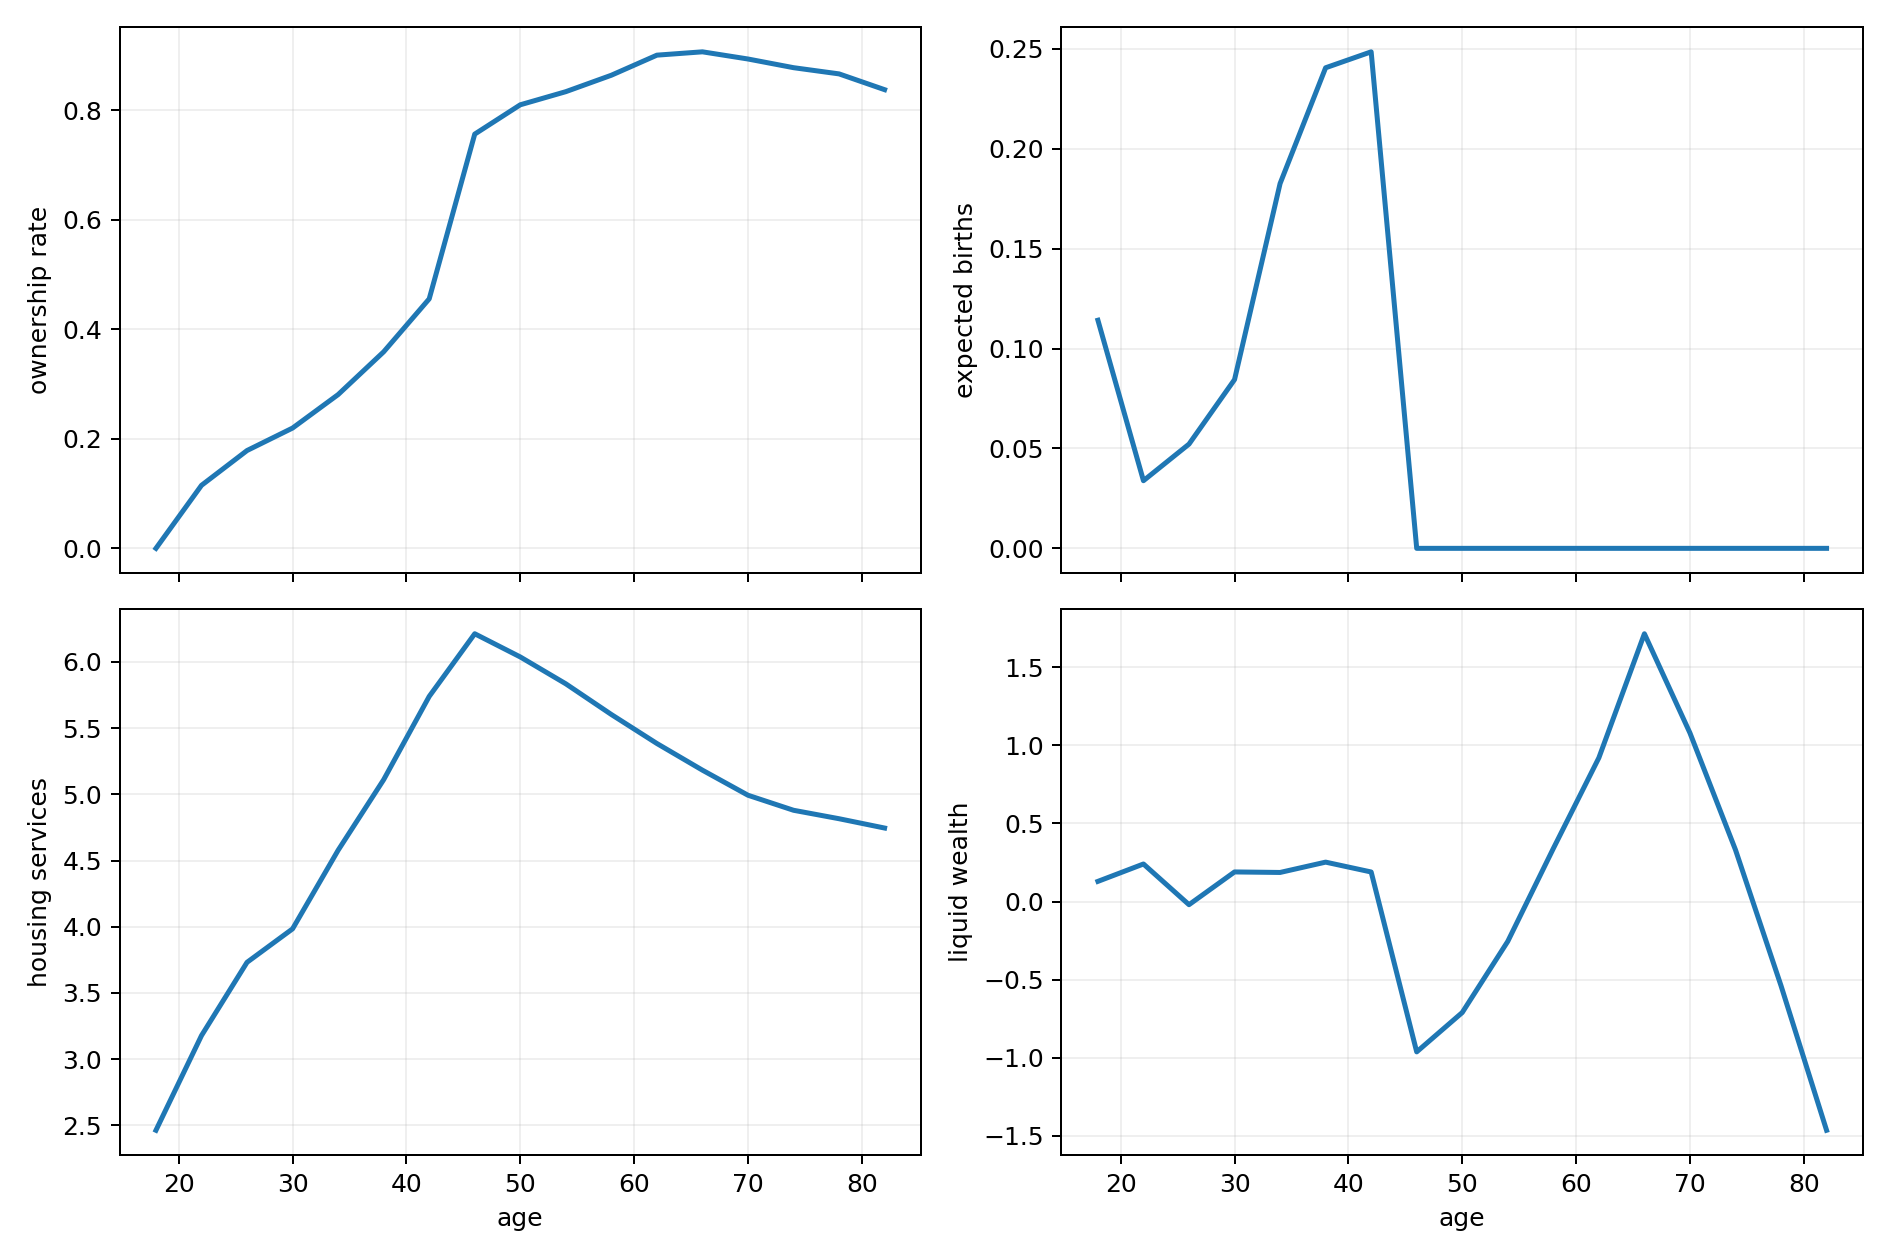
\includegraphics[width=0.97\textwidth,height=0.58\textheight,keepaspectratio]{assets/age_profiles.png}
  \begin{itemize}
    \item Ownership jumps at the last fertile age.
    \item Births occur at $33$ with a deadline spike; the data benchmark is $\sim27$.
    \item Liquid wealth falls sharply at the family purchase, consistent with maximum leverage.
  \end{itemize}
  \takeaway{The fit problem is timing: the model buys and gives birth too late.}
\end{frame}

% 15
\begin{frame}{The remaining misses point to missing mechanisms rather than a new local search}
  \begin{tabularx}{\textwidth}{>{\raggedright\arraybackslash}p{0.45\textwidth}>{\raggedright\arraybackslash}X}
  \toprule
  diagnosed miss & designed but not adopted fix\\
  \midrule
  Old-age ownership is $0.892$ in the model vs $0.764$ in the data. & Add a health, mortality, or downsizing exit margin for old owners.\\
  Young ownership is $0.226$ vs $0.341$, and young wealth is $0.354$ vs $0.179$. & Address fertility timing rather than only re-searching the same box.\\
  Childlessness by income goes the wrong way relative to the data. & Add a child time cost so children are not priced only in goods and rooms.\\
  \bottomrule
  \end{tabularx}
  \takeaway{The miss pattern is coherent: late fertility and absent old-age exit do work that parameters cannot do cleanly.}
\end{frame}

% 16
\begin{frame}{The measured access gap is the theory prediction showing up quantitatively}
  \begin{itemize}
    \item Among cap-pinned fertile renters, $\zeta/q=1.28$.
    \item These renters value family space at $2.3\times$ market user cost.
    \item $0.734$ of fertility-derivative mass sits on $\zeta>0$ households.
    \item The result is grid-converged, robust across re-weighted calibrations, and ladder-invariant.
  \end{itemize}
  The equal-scaling result says that \(\Psi_i^m\) rises with the normalized gap \(\zeta_i^m/(c_i^m-\chi n_i^m)\).
  \takeaway{This is the \(\Psi\)-proportional-to-\(\zeta\) theory prediction in the calibrated model.}
\end{frame}

% 17
\begin{frame}{Ownership is triggered by births at the deadline}
  \centering
  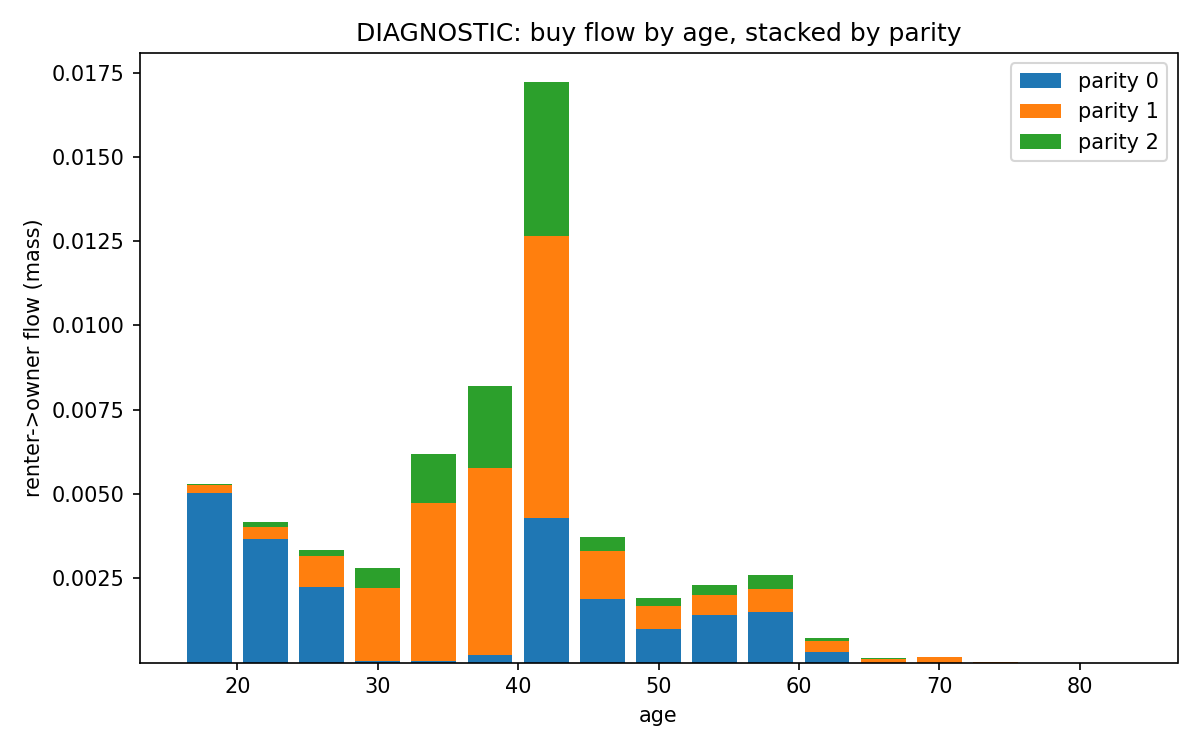
\includegraphics[width=0.88\textwidth,height=0.56\textheight,keepaspectratio]{assets/buy_flow_by_age_parity.png}
  \begin{itemize}
    \item \notfound{29 percent of the age-42 cohort buys in one period in the named source files}.
    \item \notfound{65 percent of parent buyers purchase within the birth period in the named source files}.
    \item \notfound{buyers arrive roughly 10 grid cells above the down-payment threshold in the named source files}.
  \end{itemize}
  \takeaway{The purchase margin is a birth-timing margin, not slow saving alone.}
\end{frame}

% 18
\begin{frame}{Family-sized housing is mostly held outside the fertile-parent margin}
  The calibrated allocation gives the empirical face of the misallocation proposition:
  \[
  \begin{array}{lr}
  \toprule
  \text{holder group} & \text{share of rooms}\ge6\text{ stock}\\
  \midrule
  \text{post-fertile households} & 87\%\\
  \text{households with no kids at home} & 72\%\\
  \text{fertile parents} & 12.6\%\\
  \bottomrule
  \end{array}
  \]
  The households with the largest measured access gap hold a small share of family-sized owner stock.
  \takeaway{This is the misallocation proposition's empirical face.}
\end{frame}

% 19
\begin{frame}{A price instrument capitalizes into large-home prices but barely moves births}
  \begin{itemize}
    \item The policy is a $2\%$ tax on large homes.
    \item The large-home price effect is \notfound{-12.3 percent large-home price response in the named source files}.
    \item The tax-alone fertility response is $\Delta \mathrm{TFR}=+0.004$.
    \item Robustness is reported as grid, menu, and weight invariant in the mechanism notes; the named bridge file pins the birth effect.
  \end{itemize}
  \takeaway{This instrument capitalizes into prices; it does not create births.}
\end{frame}

% 20
\begin{frame}{Birth-linked purchase grants move fertility through access}
  The grant dose-response is monotone in the access amount:
  \[
  \begin{array}{cc}
  \toprule
  \text{grant size} & \Delta \mathrm{TFR}\\
  \midrule
  0.1 & +0.01\\
  0.4 & +0.13\\
  0.58 & +0.26\\
  1.0 & +0.49\\
  \bottomrule
  \end{array}
  \]
  Prices move \notfound{roughly +1 percent grant price response in the named source files}.
  \begin{itemize}
    \item Caveat: small conditional grants can delay pre-birth purchases through anticipation effects.
  \end{itemize}
  \takeaway{Access grants move the birth margin because they relax \(\zeta_i^{O,F}\).}
\end{frame}

% 21
\begin{frame}{The policy package decentralizes the planner's reallocation}
  The package taxes the incumbent stock and uses the revenue to fund young buyers' access:
  \[
  \text{large-home tax}+\text{birth-linked purchase grant}
  \quad\Rightarrow\quad
  \Delta \mathrm{TFR}=+0.15,\quad
  \Delta p_{\text{large}}=-11\%.
  \]
  The bridge note reports this package as revenue-funded.
  \takeaway{Access, not price, is the fertility margin.}
\end{frame}

% 22
\begin{frame}{The bridge is access gaps, stock misallocation, and decentralized reallocation}
  \begin{enumerate}
    \item Measured access: capped fertile renters have \(\zeta/q=1.28\), and \(0.734\) of the derivative mass sits on \(\zeta>0\).
    \item Stock allocation: \(87\%\) of family-sized stock is held by post-fertile households.
    \item Policy: the tax-funded access transfer raises TFR by \(0.15\) while cutting large-home prices by \(11\%\).
  \end{enumerate}
  The bridge note's synthesis is that the same \(\zeta\) object measures fertility exposure and misallocation, and the package is the decentralized version of the planner reallocation.
\end{frame}

% 23
\begin{frame}{The next version needs mechanisms for bounds, timing, and childlessness}
  \begin{itemize}
    \item \notfound{8 of 13 calibrated parameters at search bounds in the named source files}.
    \item The fertility-timing issue remains: births occur at \(33\) while the data benchmark is \(\sim27\).
    \item Designed extension: add a child time cost to price children partly in foregone income.
    \item Designed extensions: add an old-age exit margin and estimand-consistent childlessness targets.
  \end{itemize}
  \takeaway{The draft should present these as limitations, not as solved calibration details.}
\end{frame}

% 24
\begin{frame}{[PLACEHOLDER: the conclusion claim is still to be written]}
  \alert{[PLACEHOLDER: conclusion]}
  \begin{itemize}
    \item [PLACEHOLDER: final theory sentence]
    \item [PLACEHOLDER: final quantitative sentence]
    \item [PLACEHOLDER: final policy sentence]
  \end{itemize}
\end{frame}

\end{document}
